\documentclass[11pt,a4paper]{article}
\usepackage[T1]{fontenc}
\usepackage[margin=2.3cm]{geometry}
\usepackage{amsmath,amssymb}
\usepackage{graphicx}
\usepackage[dvipsnames]{xcolor}
\usepackage{enumitem}
\usepackage[colorlinks=true,linkcolor=blue,urlcolor=blue]{hyperref}
\setlength{\parskip}{0.6em}
\setlength{\parindent}{0pt}
\begin{document}

\begin{center}{\LARGE\bfseries opentruss}\\[0.4em]{\large Compute the force in every bar of a truss bridge, in three sessions.}\\[0.2em]\small PAN IIT OSS explainer \textbullet{} diploma / undergraduate to advanced undergraduate (levels 5-6)\end{center}

\section*{Why this exists}
A truss is a frame of straight bars that carries load only as tension and compression. This explainer shows how engineers find those forces, from the balance of a single pin to one matrix equation for a whole bridge, using only trigonometry, force balance and a little linear algebra.

\section*{The end goal}
Compute member forces in a truss bridge. The end goal is computing member forces in a truss bridge: which bars are pulled, which are pushed, how big the forces are and how far the bridge sags. The same method sits inside structural analysis software, which is why this repo stays educational and never a design tool.

\section*{How the three sessions build up}
\begin{enumerate}[nosep]
\item \textbf{Session 1: A triangle is rigid, and bars carry only tension or compression} (Level 1, conceptual interactive model, 60 min).
\item \textbf{Session 2: Equilibrium of every pin: the method of joints and sections} (Level 2, mathematical engineering model, 75 min).
\item \textbf{Session 3: A stiffness solver for any truss, validated} (Level 3, simulation and validation, 90 min).
\end{enumerate}

\section{Session 1: A triangle is rigid, and bars carry only tension or compression}

\subsection*{A. Real-world problem}
Look under a railway bridge or at a crane arm: you see straight bars joined into triangles. Why triangles and not rectangles? And when a heavy lorry stops in the middle of a small bridge, which bars are being pulled and which are being squashed? Engineers need to know, because a pulled bar and a squashed bar fail in different ways. This session builds the picture from the simplest truss. It is an educational model, not a design method.

\subsection*{B. Concept and theory}
A truss is a set of straight bars joined at pins; the loads act only at the pins. Then every bar is pulled or pushed along its own axis and nothing else. A bar that is pulled is in tension (we write its force as positive, drawn blue). A bar that is pushed is in compression (negative, drawn red). Four pinned bars forming a rectangle can lean over into a parallelogram with all bar lengths unchanged: the rectangle is a mechanism. A triangle cannot change its angles without changing a side, so it is rigid; a frame of j joints needs at least 2 j - 3 bars. For the simplest bridge truss (two equal sloping bars meeting at a loaded apex and a bottom bar joining the feet) the supports each carry P/2. Balance of the vertical forces at the apex gives 2 F sin(theta) = P, and balance of the horizontal forces at a foot gives the bottom-bar force.

\begin{itemize}[nosep]
\item P: load at the apex (kN)
\item L: span between the supports (6 m here) (m)
\item h: height of the apex above the supports (m)
\item theta: slope angle of the sloping bars (degrees)
\item F\_top: force in each sloping bar (negative = compression) (kN)
\item F\_bot: force in the bottom bar (positive = tension) (kN)
\item j: number of joints (pins) (no unit)
\end{itemize}

\begin{equation*}
m_{\min}=2j-3\quad\text{(bars needed for a rigid frame of } j \text{ pins)}
\end{equation*}

\begin{equation*}
d^2=a^2+b^2-2ab\cos\varphi\quad\text{(diagonal of a pinned parallelogram)}
\end{equation*}

\begin{equation*}
\theta=\arctan\!\left(\frac{h}{L/2}\right)
\end{equation*}

\begin{equation*}
2F_{\mathrm{top}}\sin\theta=-P\;\Rightarrow\;F_{\mathrm{top}}=-\frac{P}{2\sin\theta}
\end{equation*}

\begin{equation*}
F_{\mathrm{bot}}=\frac{P}{2\tan\theta}
\end{equation*}

\begin{center}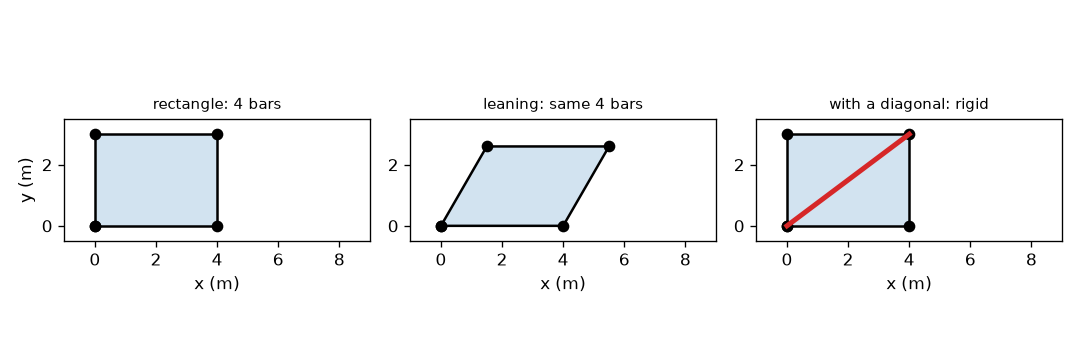
\includegraphics[width=0.85\linewidth]{figures/s01_rigid_vs_rectangle.png}\\\small A rectangle leans (same four bars); a diagonal makes it rigid.\end{center}

\subsection*{E. Worked example}
A small bridge truss spans 6 m. The apex is 3 m high and carries 10 kN. Find the force in each bar and say whether it is in tension or compression.
\begin{enumerate}[nosep]
\item Supports: by symmetry each carries 10 / 2 = 5 kN upwards.
\item Slope angle: theta = arctan(3 / 3) = 45 degrees, so sin(theta) = 0.7071 and tan(theta) = 1.
\item Apex pin, sum of vertical forces = 0: 2 F sin(45) = 10, so the size of each sloping force is 10 / (2 * 0.7071) = 7.07 kN. The bars push on the apex, so they are in compression: F\_top = -7.07 kN.
\item Left foot pin, sum of horizontal forces = 0: the sloping bar pushes the foot outwards with 7.07 * cos(45) = 5.00 kN, so the bottom bar must pull it back with 5.00 kN: F\_bot = +5.00 kN (tension).
\item Check the vertical balance at the foot: 7.07 * sin(45) = 5.00 kN, equal to the 5 kN reaction.
\end{enumerate}
\textbf{Answer.} The two sloping bars carry -7.07 kN (compression) and the bottom bar carries +5.00 kN (tension).

\subsection*{F. Questions}
\begin{enumerate}[nosep]
\item \textbf{Conceptual.} Why does adding one diagonal make a rectangle of pinned bars rigid, and why does the rectangle without it fail? Use the numbers of the 4 m by 3 m rectangle.
\item \textbf{Numerical.} A truss of span 6 m and height 1.5 m carries 12 kN at its apex. Find the force in the sloping bars and in the bottom bar, with signs.
\item \textbf{Graph and simulation interpretation.} On the force against height graph (10 kN load), what happens to the forces as the truss is made taller, from 0.5 m to 4 m? Give the forces at both ends.
\item \textbf{Design and optimisation challenge.} Design: choose the smallest height (to the nearest 0.25 m) so that the bottom bar's tension is at most 4 kN under a 10 kN load on a 6 m span. What compression does each sloping bar then carry, and what do you give up?
\end{enumerate}

\section{Session 2: Equilibrium of every pin: the method of joints and sections}

\subsection*{A. Real-world problem}
A 6 m footbridge truss carries a 10 kN load at midspan. Before any steel is cut, someone must know the force in every bar: which are pulled, which are pushed, and how big. The answer decides the size of each bar. The same pin-by-pin reasoning works for a three-bar wall bracket and for a bridge with eleven bars. This is a simplified teaching model with ideal pins and weightless bars; it is not a design method.

\subsection*{B. Concept and theory}
Take one pin. Every bar at the pin pulls on it along the bar's axis (a bar in tension pulls the pin towards the bar's other end). The pin is at rest, so the forces on it add to zero: sum Fx = 0 and sum Fy = 0. That is 2 equations per joint, so a truss with j joints gives 2 j equations. The unknowns are the m bar forces and the r support reactions. If m + r = 2 j the truss is statically determinate and the equations have exactly one solution; if m + r \textless{} 2 j it is a mechanism; if m + r \textgreater{} 2 j it has redundant bars and statics alone is not enough. The code writes the 2 j equations as one linear system and solves it. The method of sections cuts the truss in two and balances one piece: moments about the point where two cut bars meet remove their forces and leave the third. Stress is force over area, sigma = F / A, so a stress limit sigma\_allow fixes the smallest area A = \textbar{}F\textbar{} / sigma\_allow. A compression bar can also buckle (bend sideways) before it reaches that stress, so compression bars are made thicker in practice; Session 3 checks one case.

\begin{itemize}[nosep]
\item m: number of bars (no unit)
\item r: number of support reactions (pin = 2, roller = 1) (no unit)
\item j: number of joints (no unit)
\item F: bar force (tension positive) (kN)
\item R: support reaction (kN)
\item h: height of the Warren truss (side * sqrt(3) / 2) (m)
\item sigma: stress in a bar, F / A (MPa (N/mm\textasciicircum{}2))
\item A: cross-section area of a bar (mm\textasciicircum{}2)
\end{itemize}

\begin{equation*}
m+r=2j\quad\text{(statically determinate)}
\end{equation*}

\begin{equation*}
\sum F_x=0,\qquad \sum F_y=0\quad\text{at every pin}
\end{equation*}

\begin{equation*}
\begin{pmatrix}F_x\\F_y\end{pmatrix}_{\text{on pin}}=F\,(\cos\alpha,\ \sin\alpha)\quad\text{(tension pulls towards the other end)}
\end{equation*}

\begin{equation*}
F_{\mathrm{bottom}}\,h=R\cdot 3,\qquad F_{\mathrm{top}}\,h=-R\cdot 2\quad\text{(sections, moments about the joints at }x=3\text{ and }x=2\text{)}
\end{equation*}

\begin{equation*}
A=\frac{|F|}{\sigma_{\mathrm{allow}}}
\end{equation*}

\begin{center}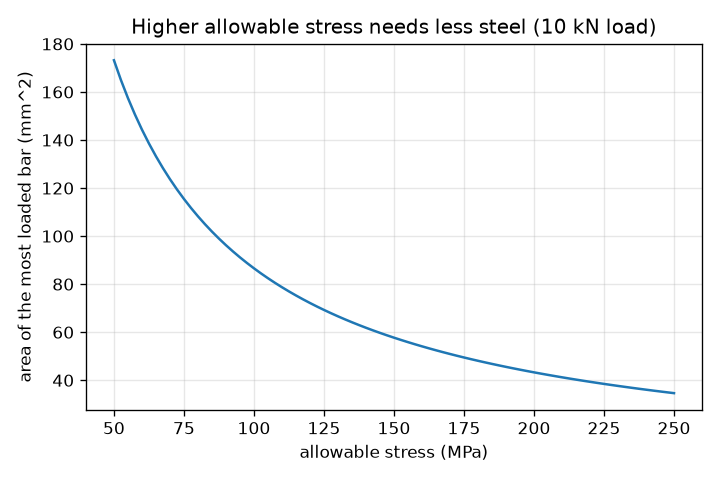
\includegraphics[width=0.85\linewidth]{figures/s02_area_vs_stress.png}\\\small Area needed by the most loaded bar against the allowable stress.\end{center}

\subsection*{E. Worked example}
A Warren truss spans 6 m with bottom joints every 2 m and equilateral triangles of side 2 m (height 1.732 m): 7 joints, 11 bars, a pin and a roller. A 10 kN load acts down at the top joint at midspan. Find the forces by joints, check one by sections, and size the most loaded bar for 150 MPa.
\begin{enumerate}[nosep]
\item Determinacy: m + r = 11 + 3 = 14 = 2 j = 14, so statics is enough.
\item Reactions: by symmetry 5 kN up at each foot, no horizontal reaction.
\item Left foot pin: the bar rising at 60 degrees gives F sin(60) + 5 = 0, so F = -5 / 0.866 = -5.77 kN (compression). Horizontal: -5.77 cos(60) + F\_bottom = 0 gives the first bottom bar +2.89 kN.
\item Next pin, the top joint above x = 1 m: the sloping bar going down to x = 2 m must carry +5.77 kN (tension) and the top chord -5.77 kN (compression). Continue pin by pin: every sloping bar is plus or minus 5.77 kN, the top chords -5.77 kN, and the middle bottom chord +8.66 kN.
\item Check by sections: cut at x = 2.5 m. Moments about the top joint at x = 3 m: F\_bottom * 1.732 = 5 * 3, so F\_bottom = +8.66 kN. Moments about the bottom joint at x = 2 m: F\_top * 1.732 = -5 * 2, so F\_top = -5.77 kN. Both agree with the joints.
\item Size the most loaded bar (8.66 kN) for 150 MPa: A = 1000 * 8.66 / 150 = 57.7 mm\textasciicircum{}2.
\end{enumerate}
\textbf{Answer.} Sloping bars +-5.77 kN, top chord -5.77 kN, bottom chord +2.89, +8.66, +2.89 kN; the most loaded bar needs 57.7 mm\textasciicircum{}2 at 150 MPa. Five bars are in tension and six in compression.

\subsection*{F. Questions}
\begin{enumerate}[nosep]
\item \textbf{Conceptual.} A truss has 12 joints, 21 bars and 3 support reactions. Is it determinate? What would you expect if one bar were removed, and what if one were added?
\item \textbf{Numerical.} Double the Warren load to 20 kN. Find the sloping bar forces and the middle bottom chord, and the area the chord needs at 150 MPa. Then round the areas up to 120 mm\textasciicircum{}2 for the chord and 80 mm\textasciicircum{}2 for the sloping bars: what are the stresses?
\item \textbf{Graph and simulation interpretation.} In the bar chart of the Warren truss, how many bars are in tension, how many in compression, and which group is the top chord in? Which bar has the largest force?
\item \textbf{Design and optimisation challenge.} Design: for the 20 kN load use bars of 120 mm\textasciicircum{}2 for the chord and 80 mm\textasciicircum{}2 for the other 10 bars, against 120 mm\textasciicircum{}2 for all 11 bars. Compare the steel volumes (all bars 2 m long) and say what the buckling concern changes.
\end{enumerate}

\section{Session 3: A stiffness solver for any truss, validated}

\subsection*{A. Real-world problem}
Statics (Session 2) breaks down when a truss has extra bars, and it says nothing about how far a bridge sags. A footbridge must be strong and stiff, so engineers use the direct stiffness method: every bar is a spring, and one matrix equation K u = f gives all the deflections and forces. Which bar shape sags least? What happens when one bar is missing? When does a slim compression bar buckle? This is a simplified educational solver: ideal pins, small deflections, never for real structures.

\subsection*{B. Concept and theory}
A bar from joint i to joint k, of length L and axial stiffness EA/L, resists changes of length. If c = cos(angle) and s = sin(angle) are the direction cosines of the bar, it adds a 4 by 4 block (EA/L) [[C, -C], [-C, C]] to the global matrix K, where C = [[c c, c s], [c s, s s]]. Assembling all bars gives K, which relates joint displacements u to joint forces f. Supports remove degrees of freedom: we keep the free ones, solve K\_ff u\_f = f\_f, then recover each bar force as F = (EA/L) (u\_k - u\_i) . (c, s) with tension positive. A mechanism has a singular K\_ff (some motion costs no energy), which shows as a rank smaller than the number of free degrees of freedom, or a huge condition number. For deflection checks, the unit-load (virtual work) formula says delta = sum of F f L / EA over all bars, where f are the bar forces for a unit load at the joint where the deflection is wanted. A compression bar can buckle: the Euler load of a pin-ended column is P\_cr = pi\textasciicircum{}2 E I / L\textasciicircum{}2, used here only as a check. For a determinate truss, bar forces do not depend on EA, and deflections are proportional to 1/EA; for an indeterminate truss, forces depend on the relative stiffness.

\begin{itemize}[nosep]
\item E: Young's modulus (steel, 200 GPa) (GPa)
\item A: bar cross-section area (mm\textasciicircum{}2)
\item EA: axial stiffness of a bar (E in GPa times A in mm\textasciicircum{}2) (kN)
\item L: bar length (m)
\item K: global stiffness matrix (kN/m)
\item u: joint displacement vector (m)
\item f: joint load vector (kN)
\item I: second moment of area of a bar section (m\textasciicircum{}4)
\item P\_cr: Euler buckling load (kN)
\end{itemize}

\begin{equation*}
k_e=\frac{EA}{L}\begin{pmatrix}C&-C\\-C&C\end{pmatrix},\quad C=\begin{pmatrix}c^2&cs\\cs&s^2\end{pmatrix}
\end{equation*}

\begin{equation*}
K\,u=f\;\Rightarrow\;K_{ff}\,u_f=f_f
\end{equation*}

\begin{equation*}
F_e=\frac{EA}{L}\,(u_k-u_i)\cdot(c,\ s)
\end{equation*}

\begin{equation*}
\delta=\sum_e \frac{F_e\,f_e\,L_e}{(EA)_e}\quad\text{(unit-load method)}
\end{equation*}

\begin{equation*}
P_{cr}=\frac{\pi^2 E I}{L^2},\qquad I=\frac{A^2}{4\pi}\ \text{(solid round bar)}
\end{equation*}

\begin{center}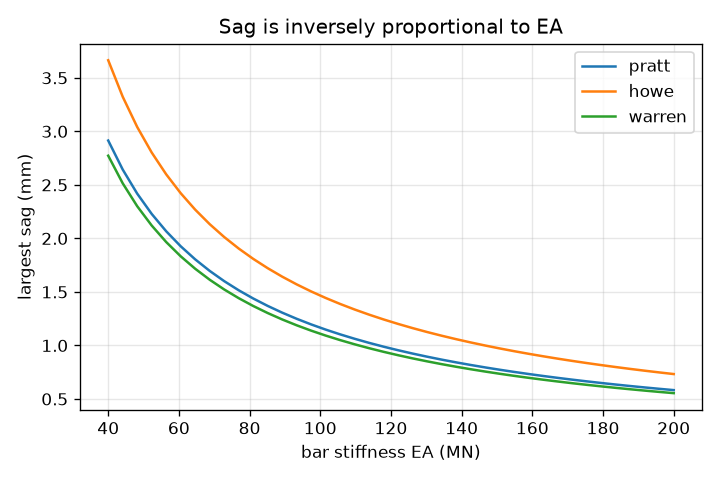
\includegraphics[width=0.85\linewidth]{figures/s03_sag_vs_ea.png}\\\small Largest sag against bar stiffness EA for the three shapes (inverse proportion).\end{center}

\subsection*{E. Worked example}
For the 8 m Pratt truss (4 panels of 2 m, height 2 m, EA = 80 000 kN for every bar, 10 kN at midspan) find the midspan sag by the unit-load method and compare it with the solver.
\begin{enumerate}[nosep]
\item Forces for 10 kN (statics): bottom chords +5 kN (4 bars, 2 m), top chords -10 kN (2 bars, 2 m), end posts -7.07 kN and diagonals +7.07 kN (4 bars of 2.83 m), verticals 0.
\item A unit load at midspan gives forces equal to these divided by 10, so F f = F\textasciicircum{}2 / 10.
\item Sum of F\textasciicircum{}2 L: bottom 4 * 25 * 2 = 200; top 2 * 100 * 2 = 400; end posts 2 * 50 * 2.828 = 282.84; diagonals 2 * 50 * 2.828 = 282.84; total 1165.69 kN\textasciicircum{}2 m.
\item Deflection: delta = 1165.69 / 10 / 80 000 = 0.001457 m = 1.457 mm.
\item The stiffness solver gives the same 1.457 mm at midspan. Doubling the EA of one bottom bar only lowers it to 1.426 mm and changes no force.
\end{enumerate}
\textbf{Answer.} The Pratt truss sags 1.457 mm at midspan by both methods; Howe sags 1.832 mm and Warren 1.386 mm under the same load.

\subsection*{F. Questions}
\begin{enumerate}[nosep]
\item \textbf{Conceptual.} In the Pratt truss the diagonals are in tension and in the Howe truss they are in compression, although both carry the same load. Why does it matter for the design which bars are pulled?
\item \textbf{Numerical.} Use the unit-load method for the three-bar triangle truss (span 6 m, height 3 m, 10 kN at the apex, EA = 80 000 kN). Give the apex sag in mm, then check with the solver.
\item \textbf{Graph and simulation interpretation.} On the sag against EA graph, why are the three curves hyperbolas (proportional to 1/EA), and what does that tell you about doubling the steel area?
\item \textbf{Design and optimisation challenge.} Design: the 12 m footbridge (6 panels, 2 m high, 6 kN/m) is sized by stress alone (150 MPa, 100 mm\textasciicircum{}2 minimum). The sag limit is 15 mm. For each shape say whether the stress-only design passes, and what the lightest shape is when the limit is enforced by scaling all areas up together.
\end{enumerate}

\section{Real-world mini-project}
\textbf{Pick the lightest truss for a 12 m footbridge.} A small footbridge spans 12 m with six panels of 2 m and a height of 2 m. The deck load is 6 kN/m, shared between the deck joints. Steel (E = 200 GPa, density 7850 kg/m\textasciicircum{}3) may be stressed to 150 MPa, no bar may be thinner than 100 mm\textasciicircum{}2, and the largest sag must not exceed 15 mm. Using \texttt{footbridge\_case} and \texttt{size\_truss} from Session 3, size a Pratt, a Howe and a Warren truss and choose the lightest. All numbers are illustrative; this is a teaching exercise, never a design for a real bridge.

\section{The path ahead}
\begin{enumerate}[nosep]
\item \textbf{Session 4: Moving loads and influence lines.} A function that places a load at any position on the deck (shared linearly between the two neighbouring deck joints) and returns the force envelope of every bar.
\item \textbf{Session 5: Buckling-aware sizing.} A sizing routine that gives compression bars a tube section and checks them against the Euler load with a safety factor.
\item \textbf{Session 6: Optimal sizing from virtual work.} A sizing routine that minimises mass for a sag limit using the unit-load formula and bounds on area.
\item \textbf{Session 7: Self-weight and load cases.} A loop that recomputes the sizing with the self-weight of the bars shared between their end joints.
\item \textbf{Session 8: Go 3D: a space truss.} The same stiffness solver for space trusses, tested on a three-legged tower (tripod).
\end{enumerate}

\section{Answers and hints}

\subsection*{Session 1}
\begin{enumerate}[nosep]
\item \textbf{Conceptual.} Hint: Compare the length of the diagonal at the 90 degree corner and at a leaning 60 degree corner. Solution: Without a diagonal, the four bar lengths stay the same when the frame leans, so nothing stops it: it is a mechanism. When it leans from 90 to 60 degrees, the distance between opposite corners changes from 5.0 m to 3.606 m. A fixed 5 m bar fixes that distance, and by the law of cosines only the 90 degree corner gives 5 m, so the frame can no longer move. A frame with 4 joints needs 2*4 - 3 = 5 bars, and the rectangle has only 4.
\item \textbf{Numerical.} Hint: tan(theta) = 1.5 / 3 = 0.5, so sin(theta) = 0.4472. Solution: F\_top = -12 / (2 * 0.4472) = -13.42 kN (compression). F\_bot = 12 / (2 * 0.5) = +12.00 kN (tension). Check: the sloping bar's vertical part is 13.42 * 0.4472 = 6.0 kN, which is half the load. Units: kN.
\item \textbf{Graph and simulation interpretation.} Hint: Read the red and blue curves at h = 0.5 and h = 4. Solution: Both curves fall as h grows. At h = 0.5 m the bars carry -30.41 kN and +30.00 kN, three times the 10 kN load. At h = 4 m they carry -6.25 kN and +3.75 kN. A flat truss is almost a straight cable-and-strut that must resist the load at a shallow angle, so the forces are huge.
\item \textbf{Design and optimisation challenge.} Hint: F\_bot = P / (2 tan theta) = P * 3 / (2 h). Solution: F\_bot = 10 * 3 / (2 h) = 15 / h \textless{}= 4 gives h \textgreater{}= 3.75 m. At h = 3.75 m the slope is 51.3 degrees, the bottom bar has exactly +4.00 kN and each sloping bar -6.40 kN. Trade-off: a taller truss reduces the forces but needs longer bars, more height clearance and more bracing against sideways wind, and long compression bars are more prone to buckling.
\end{enumerate}

\subsection*{Session 2}
\begin{enumerate}[nosep]
\item \textbf{Conceptual.} Hint: Compare m + r with 2 j. Solution: m + r = 24 = 2 j = 24, so it is determinate. Remove a bar: m + r = 23 \textless{} 24, so there are fewer unknowns than equations: the truss is a mechanism and can move (or is not in equilibrium for every load). Add a bar: m + r = 25 \textgreater{} 24, so it is statically indeterminate and statics alone cannot give the forces; stiffness is needed (Session 3).
\item \textbf{Numerical.} Hint: The truss is linear: every force doubles. Solution: Sloping bars: +-11.55 kN; middle bottom chord +17.32 kN. Chord area: 1000 * 17.32 / 150 = 115.5 mm\textasciicircum{}2; sloping bars: 1000 * 11.55 / 150 = 77.0 mm\textasciicircum{}2. With 120 mm\textasciicircum{}2 the chord stress is 17.32 * 1000 / 120 = 144.3 MPa and with 80 mm\textasciicircum{}2 the sloping bars have 11.55 * 1000 / 80 = 144.3 MPa, both below 150 MPa. Sanity check: forces doubled when the load doubled.
\item \textbf{Graph and simulation interpretation.} Hint: Blue bars point up (positive), red bars point down. Solution: Five bars are in tension (the three bottom-chord bars and two sloping bars) and six in compression (the two top-chord bars and four sloping bars). The top chord is in compression. The largest force is the middle bottom chord, +8.66 kN, because the bending-like effect of the load is largest at midspan.
\item \textbf{Design and optimisation challenge.} Hint: Volume = area * length, summed over bars; each bar is 2 m. Solution: One size: 120 * 2 * 11 = 2640 mm\textasciicircum{}2 m. Two sizes: 120 * 2 + 80 * 2 * 10 = 1840 mm\textasciicircum{}2 m, a saving of 30 percent. The saving assumes tension and compression bars are equally strong per area; compression bars can buckle at lower stresses, so in a real design they would be made larger (or as tubes) and the saving would be smaller. This model does not check buckling.
\end{enumerate}

\subsection*{Session 3}
\begin{enumerate}[nosep]
\item \textbf{Conceptual.} Hint: Think about which failure a slim bar suffers in tension and which in compression. Solution: A bar in tension fails only when its stress reaches the material limit, so a thin bar is fine. A bar in compression can buckle at a much lower force (Euler: P\_cr falls with the square of its length). The Pratt shape puts the long diagonals in tension and the short verticals in compression (here they carry zero under the midspan load), so it is usually the sounder choice for steel; Howe puts the long diagonals in compression.
\item \textbf{Numerical.} Hint: Forces: -7.07, -7.07 and +5.00 kN; unit-load forces are one tenth of these; the sloping bars are 4.243 m long, the bottom bar 6 m. Solution: Sum F f L / EA = (2 * 7.07 * 0.707 * 4.243 + 5 * 0.5 * 6) / 80 000 = (42.43 + 15) / 80 000 = 0.000718 m = 0.718 mm. The solver gives the same 0.718 mm downwards.
\item \textbf{Graph and simulation interpretation.} Hint: Look at the formula delta = sum F f L / EA for a determinate truss. Solution: The forces F and f do not depend on EA in a determinate truss, so delta is a constant divided by EA: doubling every bar's area halves the sag. The curves are ordered Howe above Pratt above Warren, and they never cross. The bar forces do not change: stiffness only moves the deflection.
\item \textbf{Design and optimisation challenge.} Hint: Use \texttt{footbridge\_case} and \texttt{size\_truss} with \texttt{limit\_mm=15.0}. Solution: Stress-only designs sag 21.8 mm (Pratt), 25.4 mm (Howe) and 22.7 mm (Warren): all fail. Scaling the areas up by 1.45, 1.69 and 1.51 gives sags of exactly 15.0 mm, with masses 111 kg (Pratt), 136 kg (Howe) and 115 kg (Warren): the Pratt truss is lightest. Assumptions: uniform scale-up (not optimal sizing), 7850 kg/m\textasciicircum{}3 steel, no buckling check, illustrative numbers.
\end{enumerate}

\section{How to join}
Read \texttt{CONTRIBUTING.md} in the repository, then pick an issue labelled \texttt{good first issue}. Repository: \url{https://github.com/KrunalPanchal1995/opentruss}

\end{document}
